\documentclass[paper=screen,mathserif]{beamer}\usepackage[]{graphicx}\usepackage[]{color}
%% maxwidth is the original width if it is less than linewidth
%% otherwise use linewidth (to make sure the graphics do not exceed the margin)
\makeatletter
\def\maxwidth{ %
  \ifdim\Gin@nat@width>\linewidth
    \linewidth
  \else
    \Gin@nat@width
  \fi
}
\makeatother

\definecolor{fgcolor}{rgb}{0.345, 0.345, 0.345}
\newcommand{\hlnum}[1]{\textcolor[rgb]{0.686,0.059,0.569}{#1}}%
\newcommand{\hlstr}[1]{\textcolor[rgb]{0.192,0.494,0.8}{#1}}%
\newcommand{\hlcom}[1]{\textcolor[rgb]{0.678,0.584,0.686}{\textit{#1}}}%
\newcommand{\hlopt}[1]{\textcolor[rgb]{0,0,0}{#1}}%
\newcommand{\hlstd}[1]{\textcolor[rgb]{0.345,0.345,0.345}{#1}}%
\newcommand{\hlkwa}[1]{\textcolor[rgb]{0.161,0.373,0.58}{\textbf{#1}}}%
\newcommand{\hlkwb}[1]{\textcolor[rgb]{0.69,0.353,0.396}{#1}}%
\newcommand{\hlkwc}[1]{\textcolor[rgb]{0.333,0.667,0.333}{#1}}%
\newcommand{\hlkwd}[1]{\textcolor[rgb]{0.737,0.353,0.396}{\textbf{#1}}}%

\usepackage{framed}
\makeatletter
\newenvironment{kframe}{%
 \def\at@end@of@kframe{}%
 \ifinner\ifhmode%
  \def\at@end@of@kframe{\end{minipage}}%
  \begin{minipage}{\columnwidth}%
 \fi\fi%
 \def\FrameCommand##1{\hskip\@totalleftmargin \hskip-\fboxsep
 \colorbox{shadecolor}{##1}\hskip-\fboxsep
     % There is no \\@totalrightmargin, so:
     \hskip-\linewidth \hskip-\@totalleftmargin \hskip\columnwidth}%
 \MakeFramed {\advance\hsize-\width
   \@totalleftmargin\z@ \linewidth\hsize
   \@setminipage}}%
 {\par\unskip\endMakeFramed%
 \at@end@of@kframe}
\makeatother

\definecolor{shadecolor}{rgb}{.97, .97, .97}
\definecolor{messagecolor}{rgb}{0, 0, 0}
\definecolor{warningcolor}{rgb}{1, 0, 1}
\definecolor{errorcolor}{rgb}{1, 0, 0}
\newenvironment{knitrout}{}{} % an empty environment to be redefined in TeX

\usepackage{alltt}

\usetheme{CambridgeUS} 
\useinnertheme{circles}
\useoutertheme[footline=authortitle,subsection = false]{miniframes}
\setbeamercolor{palette tertiary}{fg=white, bg=white!42!black}
\setbeamercolor{alerted text}{fg=red!73!black}

%%%%%%
%\usepackage{Sweave}
\usepackage{natbib}     % for references
\usepackage[osf]{sourcesanspro}
%\usepackage{sourcecodepro}
\usepackage{booktabs}
\usepackage{dcolumn}
\usepackage{eulervm}
%\renewcommand{\ttdefault}{sourcecodepro}
\usepackage{import}
\usepackage{prodint}
\usepackage{bbm}
\usepackage{tabularx}
\usepackage{dcolumn}
\usepackage{color}
\usepackage{booktabs}
\usepackage{graphicx,rotating,epsfig,multirow,multicol,hhline}
\usepackage{amsmath,amsthm,amssymb,amsfonts}

\newcommand{\subfloat}[2][need a sub-caption]{\subcaptionbox{#1}{#2}}

\usepackage{listings}
\lstset{
  basicstyle=\tiny\ttfamily, % Standardschrift
  % numbers=left,               % Ort der Zeilennummern
  %numberstyle=\tiny,          % Stil der Zeilennummern
  % stepnumber=2,               % Abstand zwischen den Zeilennummern
  numbersep=5pt,              % Abstand der Nummern zum Text
  tabsize=2,                  % Groesse von Tabs
  extendedchars=true,         %
  breaklines=true,            % Zeilen werden Umgebrochen
  keywordstyle=\color{blue},
  frame=b,         
  stringstyle=\color{white}\ttfamily, % Farbe der String
  showspaces=false,           % Leerzeichen anzeigen ?
  showtabs=false,             % Tabs anzeigen ?
}

\usepackage{subcaption}

\newcommand{\ft}[1]{\frametitle{#1}}
\newcommand{\fst}[1]{\framesubtitle{#1}}

\title[Some more \LaTeX]{Introduction to Biostatistical Computing}
\subtitle{A bit more on \LaTeX}

\author{Arthur Allignol}

\institute[]{\scriptsize{\url{arthur.allignol@uni-ulm.de}}}

\date{}
%%%%%%
\makeatletter
\setbeamertemplate{footline}
{
  \leavevmode%
  \hbox{%
  \begin{beamercolorbox}[wd=.333333\paperwidth,ht=2.25ex,dp=1ex,center]{author in head/foot}%
    \usebeamerfont{author in head/foot}\insertshortauthor%~~\beamer@ifempty{\insertshortinstitute}{}{(\insertshortinstitute)}
  \end{beamercolorbox}%
  \begin{beamercolorbox}[wd=.333333\paperwidth,ht=2.25ex,dp=1ex,center]{title in head/foot}%
    \usebeamerfont{title in head/foot}\insertshorttitle
  \end{beamercolorbox}%
  \begin{beamercolorbox}[wd=.333333\paperwidth,ht=2.25ex,dp=1ex,right]{date in head/foot}%
    \usebeamerfont{date in head/foot}\insertshortdate{}\hspace*{2em}
    \insertframenumber\hspace*{2ex} 
  \end{beamercolorbox}}%
  \vskip0pt%
}
\makeatother


\AtBeginSection[]
{
  \begin{frame}
    \frametitle{Table of Contents}
    \tableofcontents[currentsection]
  \end{frame}
}
\IfFileExists{upquote.sty}{\usepackage{upquote}}{}
\begin{document}

%%%%%% title page
\newcommand{\titlep}{yes}  % for titlepagelayout

{
\renewcommand{\insertframenumber}{}   % no page number on titlepage
\begin{frame}
\addtocounter{framenumber}{-1}
\titlepage
\end{frame}
}




\section{Introduction}

\begin{frame}
  \ft{What is \TeX{}/\LaTeX?}
  \begin{description}
    \item[\TeX] is a programming language (and also a typesetting
      system) written by Donald Knuth; released in 1978
    \item[\LaTeX] is a macro package facilitating the use of of \TeX
  \end{description}
  \vspace{0.5cm}
  {\bf Installation}
  \begin{description}
  \item[Windows] MiKTeX \url{http://www.miktex.org/}
  \item[OSX] MacTex \url{http://www.tug.org/mactex/}
  \item[Linux/UNIX] TeX Live \url{http://www.tug.org/texlive/}
  \end{description}

\end{frame}

\begin{frame}[fragile]
  \ft{Minimal \LaTeX{} document}
  
\begin{verbatim}
\documentclass{article}

\begin{document}

Hello World!

\end{document}
\end{verbatim}
\end{frame}

\begin{frame}[fragile]
  \ft{A usual \LaTeX{} document}
  
\begin{verbatim}
\documentclass{article}  |
\usepackage{color}       |
\usepackage{graphicx}    |
                         |  Preamble (options)
\title{A Title}          |
\author{John Doe}        |
\date{\today}            |
                         |
\begin{document}         |

\maketitle

Hello World!

\end{document}

everything below is ignored

\end{verbatim}
\end{frame}

\begin{frame}[fragile]
  \ft{{\tt \textbackslash documentclass[options]\{class\}}}
  
  Can be used with or without options
  
{\scriptsize 
\begin{verbatim}
\documentclass[10pt]{article}          % 10pt|11pt|12pt
\documentclass[final]{article}         % draft|final
\documentclass[a4paper]{article}       % a4paper|a5paper|letterpaper|...
\documentclass[twoside]{book}          % oneside|twoside
\documentclass[openright]{book}        % openright|openany
\documentclass[notitlepage]{article}   % notitlepalge|titlepage
\documentclass[onecolumn]{article}     % onecolumn|twocolumn
\documentclass[a4paper,oneside,12pt]{article} % combined  with comma
\end{verbatim}
}
  
\end{frame}

\begin{frame}[fragile]
  \ft{Sectioning and table of content}
  
  \begin{itemize}
  \item Section are declared using
\begin{verbatim}
\section{Section's title}
\end{verbatim}
  \item Other sectioning commands are
    \begin{itemize}
    \item \verb=\chapter=
    \item \verb=\part=
    \item \verb=subsection=
    \item \verb=subsubsection=
    \item \verb=\paragraph=
    \end{itemize}

  \item A \verb=\tableofcontents= command produces a table of contents
    
  \end{itemize}
  
\end{frame}

\section{Newcommands}

\begin{frame}[fragile]
  \frametitle{\LaTeX{} Commands and Newcommands}
  Various builtin commands (macros) in \LaTeX
  \begin{itemize}
  \item Commands start with \textbackslash
  \item May have arguments, e.g., \verb+\section{Newcommands}+
  \item or none, e.g., \verb|\LaTeX| (that produces \LaTeX)
  \end{itemize}\vspace{0.3cm}
  In addition, the user may define his own commands. Useful for nasty
  expressions that appear often
  \begin{itemize}
  \item \verb|\newcommand{\keyword}{definition}|
  \item A \verb=newcommand= definition may appear anywhere in a .tex
    file (though usually defined in the preamble)
  \item A \verb=\newcommand= keyword may not contain numbers
  \end{itemize}
\end{frame}

\begin{frame}[fragile]
  \frametitle{Newcommands}
  
  \newcommand{\com}{My command}
  \newcommand{\Z}{\mathbb{Z}}
  
  \begin{block}{Example}
\begin{verbatim}
\newcommand{\com}{My command}
My first newcommand \com
\end{verbatim}
    \begin{itemize}
    \item My first newcommand \com
    \end{itemize}
\begin{verbatim}
\newcommand{\Z}{\mathbb{Z}}
For $k \in \Z$
\end{verbatim}
    \begin{itemize}
    \item For $k \in \Z$. Note that it works in math mode
    \end{itemize}
    \renewcommand{\Z}{\ensuremath{\mathbb{Z}}}
\begin{verbatim}
\newcommand{\Z}{\ensuremath{\mathbb{Z}}}
Both $\Z$ and \Z{} work
\end{verbatim}
    \begin{itemize}
    \item Both $\Z$ and \Z{} work
    \end{itemize}
  \end{block}
\end{frame}

\begin{frame}[fragile]
  \ft{Newcommands with arguments}
  
  \begin{itemize}
  \item User-defined commands may receive arguments
    \begin{block}{}
\begin{verbatim}
\newcommand{\keyword}[n]{definition}
\end{verbatim}
    \end{block}
    where \verb=n= is the number of arguments (1-9)
\item One refers to arguments in the definition using \verb=#k=,
  \verb=k= $=1, \dots, n$
\item Default values for possible optional arguments can be given
  using the form
  \begin{block}{}
\begin{verbatim}
\newcommand{\keyword}[n][default]{definition}
\end{verbatim}
  \end{block}
\item Existing commands may be redefined using \verb=\renewcommand=
  in a similar way
\end{itemize}
\end{frame}

\begin{frame}[fragile]
  \ft{Newcommand with arguments}
  
  \newcommand{\norm}[1]{\lVert#1\rVert}
  \newcommand{\subvec}[3]{\ensuremath{#1_{#2},\ldots,#1_{#3}}}
  
  \begin{block}{}
\begin{verbatim}
\newcommand{\norm}[1]{\lVert#1\rVert}
$\norm{f + g} \leq \norm{f} + \norm{g}$
\end{verbatim}
    \begin{itemize}
    \item $\norm{f + g} \leq \norm{f} + \norm{g}$
    \end{itemize}
\begin{verbatim}
\newcommand{\subvec}[3]{\ensuremath{#1_{#2},\ldots,#1_{#3}}}
\subvec{a}{1}{n}
\subvec{a}{ij}{kl}
\end{verbatim}
    \begin{itemize}
    \item \subvec{a}{1}{n}
    \item \subvec{a}{ij}{kl}
    \end{itemize}
    
  \end{block}
\end{frame}

\section{Tables, Graphics and Floats}

\begin{frame}[fragile]
  \ft{Tables}
  \fst{The {\tt tabular} Environment}
  \begin{itemize}
  \item Columns separated by {\tt \&}
  \item Rows separated by \verb=\\=
  \item Environment argument is column formatting specification
    \begin{description}
    \item[{\tt c}] centered
    \item[l] flush left
    \item[r] flush right
    \item[{\tt p\{2.5cm\}}] limit column width (left aligned)
    \end{description}
  \item A \verb+|+ {\tt tabular}'s environment puts a vertical line at
    the specified place
  \item The \verb=\hline= command draws a horizontal line
  \item The \verb=\cline{i-j}= command draws a horizontal line between
    the $i$th and $j$th columns
  \end{itemize}
\end{frame}

\begin{frame}[fragile]
  \ft{Tables}
  \fst{The {\tt tabular} Environment}
  \begin{block}{}
  \begin{columns}
    \begin{column}{5cm}
\scriptsize{
\begin{verbatim}
\begin{tabular}{lccc}
       & Coef & SE    & p-value \\
Age    & 0.01 & 0.002 & 0.5     \\
Gender & 2    & 1     & 0.23    \\
\end{tabular}
\end{verbatim}}
    \end{column}
    \begin{column}{5cm}
      \begin{tabular}{lccc}
               & Coef & SE    & p-value \\
        Age    & 0.01 & 0.002 & 0.5     \\
        Gender & 2    & 1     & 0.23    \\
      \end{tabular}
    \end{column}
  \end{columns}
\end{block}
  \begin{block}{}
  \begin{columns}
    \begin{column}{5cm}
\scriptsize{
\begin{verbatim}
\begin{tabular}{l|ccc}
       & Coef & SE    & p-value \\
\hline
Age    & 0.01 & 0.002 & 0.5     \\
Gender & 2    & 1     & 0.23    \\
\hline
\end{tabular}
\end{verbatim}}
    \end{column}
    \begin{column}{5cm}
      \begin{tabular}{l|ccc}
               & Coef & SE    & p-value \\
               \hline
        Age    & 0.01 & 0.002 & 0.5     \\
        Gender & 2    & 1     & 0.23    \\
        \hline
      \end{tabular}
    \end{column}
  \end{columns}
\end{block}
\end{frame}

\begin{frame}[fragile]
  \ft{Tables}
  \fst{The {\tt tabular} Environment}
  \begin{itemize}
  \item Text spanning multiple column is typeset using
    \verb=\multicolumn{num}{align}{text}=
    \begin{description}
    \item[{\tt num}] specifies the number of merged column
    \item[{\tt align}] specifies the alignment ({\tt l}, {\tt c}, {\tt
      r})
    \end{description}
  \end{itemize}
  \begin{block}{}
    \begin{columns}
      \begin{column}{5cm}
        {\scriptsize
\begin{verbatim}
\begin{tabular}{l|ccc}
  & \multicolumn{3}{c}{Regression} \\
  \cline{2-4}
  & Coef & SE    & p-value         \\
  \hline
  Age    & 0.01 & 0.002 & 0.5      \\
  Gender & 2    & 1     & 0.23     \\
  \hline
\end{tabular}
\end{verbatim}
        }
      \end{column}
      \begin{column}{5cm}
        \begin{tabular}{l|ccc}
                 & \multicolumn{3}{c}{Regression} \\
          \cline{2-4}
                 & Coef & SE    & p-value                \\
          \hline
          Age    & 0.01 & 0.002 & 0.5                    \\
          Gender & 2    & 1     & 0.23                   \\
          \hline
\end{tabular}
      \end{column}

    \end{columns}
  \end{block}
\end{frame}

\begin{frame}[fragile]
  \ft{Tables}
  \fst{The booktabs package}
  The booktabs package define the new commands
  \begin{itemize}
  \item {\tt \textbackslash toprule} to be used just after \verb=\begin{tabular}=
  \item {\tt \textbackslash midrule} to be used after variable definition
  \item {\tt \textbackslash bottomrule} to be used just before \verb=\end{tabular}=
  \item {\tt \textbackslash cmidrule} equivalent to \verb=\cline=
  \end{itemize}
  \begin{block}{}
    \begin{columns}
      \begin{column}{5cm}
        {\scriptsize
\begin{verbatim}
\begin{tabular}{lccc}
\toprule
& \multicolumn{3}{c}{Regression} \\
\cmidrule(r){2-4}
& Coef & SE    & p-value         \\
\midrule
Age    & 0.01 & 0.002 & 0.5      \\
Gender & 2    & 1     & 0.23     \\
\bottomrule
\end{tabular}
\end{verbatim}}
      \end{column}
      \begin{column}{6cm}
        \begin{tabular}{lccc}
          \toprule
           & \multicolumn{3}{c}{Regression} \\
    \cmidrule(r){2-4}
           & Coef & SE    & p-value         \\
    \midrule
    Age    & 0.01 & 0.002 & 0.5             \\
    Gender & 2    & 1     & 0.23            \\
    \bottomrule
  \end{tabular}
\end{column}
\end{columns}
\end{block}
\end{frame}

\begin{frame}[fragile]
  \ft{Tables}
  \fst{Nicer Figures with {\tt xtable}}
\begin{knitrout}\scriptsize
\definecolor{shadecolor}{rgb}{0.969, 0.969, 0.969}\color{fgcolor}\begin{kframe}
\begin{alltt}
\hlkwd{library}\hlstd{(xtable)}

\hlstd{my_xtable} \hlkwb{<-} \hlkwa{function}\hlstd{(}\hlkwc{x}\hlstd{,} \hlkwc{file} \hlstd{=} \hlstr{""}\hlstd{,}
                      \hlkwc{rownames} \hlstd{=} \hlnum{FALSE}\hlstd{,}
                      \hlkwc{colnames} \hlstd{=} \hlnum{TRUE}\hlstd{,} \hlkwc{...}\hlstd{) \{}
    \hlstd{tab} \hlkwb{<-} \hlstd{xtable}\hlopt{::}\hlkwd{xtable}\hlstd{(x, ...)}
    \hlkwd{print}\hlstd{(tab,} \hlkwc{floating} \hlstd{=} \hlnum{FALSE}\hlstd{,} \hlkwc{hline.after} \hlstd{=} \hlkwa{NULL}\hlstd{,}
          \hlkwc{add.to.row} \hlstd{=} \hlkwd{list}\hlstd{(}\hlkwc{pos} \hlstd{=} \hlkwd{list}\hlstd{(}\hlopt{-}\hlnum{1}\hlstd{,}\hlnum{0}\hlstd{,} \hlkwd{nrow}\hlstd{(x)),}
              \hlkwc{command} \hlstd{=} \hlkwd{c}\hlstd{(}\hlstr{'\textbackslash{}\textbackslash{}toprule\textbackslash{}n '}\hlstd{,}
                  \hlstr{'\textbackslash{}\textbackslash{}midrule\textbackslash{}n '}\hlstd{,}
              \hlstr{'\textbackslash{}\textbackslash{}bottomrule\textbackslash{}n'}\hlstd{)),}
          \hlkwc{file} \hlstd{= file,}
          \hlkwc{include.rownames} \hlstd{= rownames,}
          \hlkwc{include.colnames} \hlstd{= colnames)}
\hlstd{\}}
\end{alltt}
\end{kframe}
\end{knitrout}
\end{frame}

\begin{frame}[fragile]
  \ft{Tables}
  \fst{Nicer Figures with {\tt xtable}}
\begin{kframe}
\begin{alltt}
\hlstd{fit_lm} \hlkwb{<-} \hlkwd{lm}\hlstd{(life} \hlopt{~} \hlkwd{log}\hlstd{(phys)} \hlopt{+} \hlkwd{log}\hlstd{(tv),} \hlkwc{data} \hlstd{= tele)}
\hlkwd{my_xtable}\hlstd{(}\hlkwd{summary}\hlstd{(fit_lm)}\hlopt{$}\hlstd{coefficients,}
          \hlkwc{rownames} \hlstd{=} \hlnum{TRUE}\hlstd{)}
\end{alltt}
\end{kframe}% latex table generated in R 3.2.0 by xtable 1.7-4 package
% Tue Apr 28 14:56:01 2015
\begin{tabular}{rrrrr}
  \toprule
  & Estimate & Std. Error & t value & Pr($>$$|$t$|$) \\ 
  \midrule
 (Intercept) & 90.62 & 4.36 & 20.81 & 0.00 \\ 
  log(phys) & -2.26 & 0.75 & -3.02 & 0.00 \\ 
  log(tv) & -2.92 & 0.59 & -4.94 & 0.00 \\ 
   \bottomrule
\end{tabular}

\end{frame}

\begin{frame}[fragile]
  \ft{Tables with the {\bf stargazer} package}
  
\begin{kframe}
\begin{alltt}
\hlstd{fit_lm2} \hlkwb{<-} \hlkwd{lm}\hlstd{(life} \hlopt{~} \hlkwd{log}\hlstd{(tv),} \hlkwc{data} \hlstd{= tele)}
\hlkwd{stargazer}\hlstd{(fit_lm2, fit_lm,} \hlkwc{title} \hlstd{=} \hlstr{"Results"}\hlstd{,}
          \hlkwc{ci} \hlstd{=} \hlnum{TRUE}\hlstd{,} \hlkwc{font.size} \hlstd{=} \hlstr{"scriptsize"}\hlstd{)}
\end{alltt}
\end{kframe}
% Table created by stargazer v.5.1 by Marek Hlavac, Harvard University. E-mail: hlavac at fas.harvard.edu
% Date and time: Tue, Apr 28, 2015 - 02:56:01 PM
\begin{table}[!htbp] \centering 
  \caption{Results} 
  \label{} 
\scriptsize 
\begin{tabular}{@{\extracolsep{5pt}}lcc} 
\\[-1.8ex]\hline 
\hline \\[-1.8ex] 
 & \multicolumn{2}{c}{\textit{Dependent variable:}} \\ 
\cline{2-3} 
\\[-1.8ex] & \multicolumn{2}{c}{life} \\ 
\\[-1.8ex] & (1) & (2)\\ 
\hline \\[-1.8ex] 
 log(phys) &  & $-$2.259$^{***}$ \\ 
  &  & ($-$3.724, $-$0.794) \\ 
  & & \\ 
 log(tv) & $-$4.260$^{***}$ & $-$2.916$^{***}$ \\ 
  & ($-$5.103, $-$3.416) & ($-$4.073, $-$1.758) \\ 
  & & \\ 
 Constant & 77.887$^{***}$ & 90.622$^{***}$ \\ 
  & (75.496, 80.279) & (82.085, 99.159) \\ 
  & & \\ 
\hline \\[-1.8ex] 
Observations & 38 & 38 \\ 
R$^{2}$ & 0.731 & 0.787 \\ 
Adjusted R$^{2}$ & 0.724 & 0.775 \\ 
Residual Std. Error & 4.101 (df = 36) & 3.704 (df = 35) \\ 
F Statistic & 97.938$^{***}$ (df = 1; 36) & 64.598$^{***}$ (df = 2; 35) \\ 
\hline 
\hline \\[-1.8ex] 
\textit{Note:}  & \multicolumn{2}{r}{$^{*}$p$<$0.1; $^{**}$p$<$0.05; $^{***}$p$<$0.01} \\ 
\end{tabular} 
\end{table} 


\end{frame}

\begin{frame}[fragile]
  \ft{Tables with the {\bf texreg} package}
  
\begin{kframe}
\begin{alltt}
\hlkwd{texreg}\hlstd{(}\hlkwd{list}\hlstd{(fit_lm2, fit_lm),}
       \hlkwc{booktabs} \hlstd{=} \hlnum{TRUE}\hlstd{,} \hlkwc{dcolumn} \hlstd{=} \hlnum{TRUE}\hlstd{,}
       \hlkwc{use.packages} \hlstd{=} \hlnum{FALSE}\hlstd{)}
\end{alltt}
\end{kframe}
\begin{table}
\begin{center}
\begin{tabular}{l D{.}{.}{2.5}@{} D{.}{.}{2.5}@{} }
\toprule
            & \multicolumn{1}{c}{Model 1} & \multicolumn{1}{c}{Model 2} \\
\midrule
(Intercept) & 77.89^{***} & 90.62^{***} \\
            & (1.22)      & (4.36)      \\
log(tv)     & -4.26^{***} & -2.92^{***} \\
            & (0.43)      & (0.59)      \\
log(phys)   &             & -2.26^{**}  \\
            &             & (0.75)      \\
\midrule
R$^2$       & 0.73        & 0.79        \\
Adj. R$^2$  & 0.72        & 0.77        \\
Num. obs.   & 38          & 38          \\
\bottomrule
\multicolumn{3}{l}{\scriptsize{$^{***}p<0.001$, $^{**}p<0.01$, $^*p<0.05$}}
\end{tabular}
\caption{Statistical models}
\label{table:coefficients}
\end{center}
\end{table}


\end{frame}


\begin{frame}[fragile]
  \ft{Graphics}
  \begin{itemize}
  \item Graphics file are imported using the {\tt graphicx} package
    and the command \verb=\includegraphics{file}=
  \item {\tt pdflatex} allows JPG, PNG or PDF graphic formats
  \end{itemize}
  \begin{columns}
    \begin{column}{8cm}
      \begin{block}{}
        \scriptsize{
\begin{verbatim}
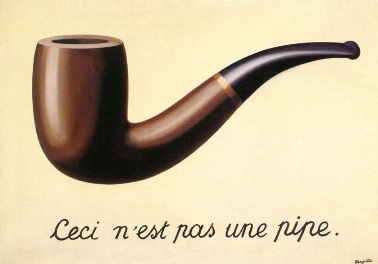
\includegraphics{graphics/MagrittePipe.jpg}
\end{verbatim}}
      \end{block}
    \end{column}
    \begin{column}{3cm}
      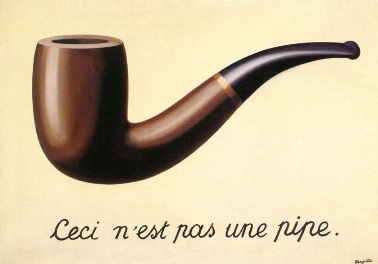
\includegraphics[width = \linewidth]{graphics/MagrittePipe}
    \end{column}
  \end{columns}
\end{frame}

\begin{frame}[fragile]
  \ft{Graphics}
  \fst{Width of figure}
  \begin{itemize}
  \item Optional argument in \verb+\includegraphics[width = opt]{file}+
    \begin{itemize}
    \item {\tt Xunit}: e.g, 5cm, 4in
    \item {\tt width=\textbackslash linewidth}: width of a line in the local
      environment
    \item {\tt width=\textbackslash textwidth}: width of the text in a page 
    \end{itemize}
  \item Also \verb+width=.5\linewidth+ or \verb+width=.5\pagewidth+
  \end{itemize}
\end{frame}

\begin{frame}[fragile]
  \ft{Graphics}
  \fst{Rotation}
  \begin{columns}
    \begin{column}{7cm}
      \begin{block}{}
        \scriptsize{
\begin{verbatim}
\includegraphics[angle=90]{graphics/
         MagrittePipe.jpg}
\end{verbatim}}
      \end{block}
    \end{column}
    \begin{column}{3cm}
      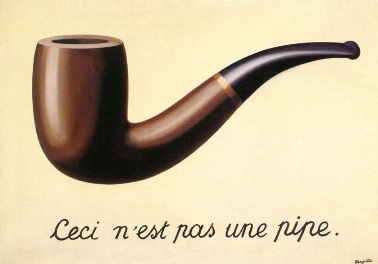
\includegraphics[angle=90,width = \linewidth]{graphics/MagrittePipe}
    \end{column}
  \end{columns}
\end{frame}

\begin{frame}[fragile]
  \ft{Graphics}
  \fst{Multiple Figures (no floating)}
  \begin{block}{}
{\scriptsize
\begin{verbatim}
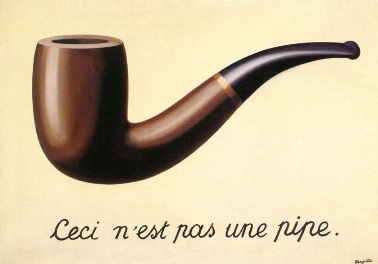
\includegraphics[width = .4\linewidth]{graphics/MagrittePipe}
\hrulefill
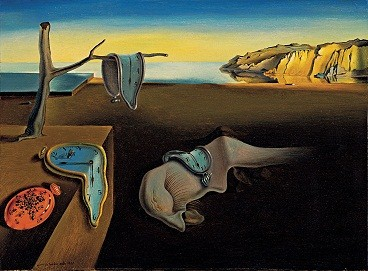
\includegraphics[width = .4\linewidth]{graphics/The_Persistence_of_Memory.jpg}
\end{verbatim}}
  \end{block}
  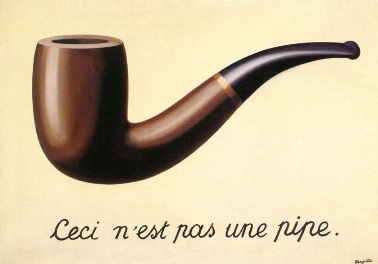
\includegraphics[width = .4\linewidth]{graphics/MagrittePipe}
  \hrulefill
  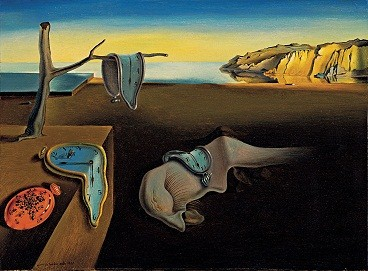
\includegraphics[width = .4\linewidth]{graphics/The_Persistence_of_Memory.jpg}
\end{frame}

\begin{frame}[fragile]
  \ft{Floating Objects}
  \begin{itemize}
  \item Sentences are broken across pages but pictures and tables
    cannot be split. They must be ``floated'' to convenient
    places. These objects are named {\em floating objects}
  \item \LaTeX{} provide two ``floating'' environments
    \begin{description}
    \item[{\tt table}] \verb=\begin{table} ... \end{table}= usually
      combined with the {\tt tabular} environment
    \item[{\tt figure}] \verb=\begin{figure} ... \end{figure}= usually
      for graphics
    \end{description}
  \item Optional arguments {\em suggests} a position for a float
    \begin{description}
    \item[{\tt h}] here
    \item[{\tt t}] top of the page
    \item[{\tt b}] bottom of the page
    \item[{\tt p}] separate page of floats
    \item[{\tt !}] strong recommendation
    \end{description}
  \end{itemize}
\end{frame}

\begin{frame}[fragile]
  \ft{Floating Objects}
  \fst{{\tt figure} environment}
  \begin{block}{}
\begin{verbatim}
\begin{figure}[ht]
  \centering
  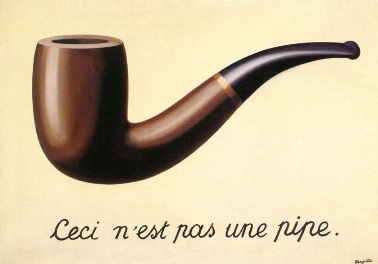
\includegraphics[width=.5\linewidth]{graphics/MagrittePipe}
\end{figure}
\end{verbatim}
  \end{block}
  \begin{figure}[ht]
    \centering
    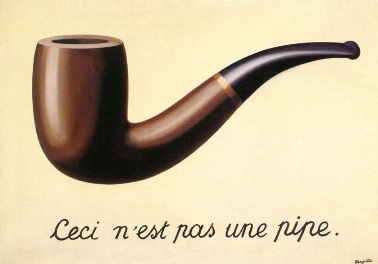
\includegraphics[width=.5\linewidth]{graphics/MagrittePipe}
  \end{figure}
\end{frame}

\begin{frame}[fragile]
  \ft{Floating Objects}
  \fst{{\tt figure} environment}
  \begin{block}{}
{\tiny 
\begin{verbatim}
\begin{figure}[ht]
  \centering
  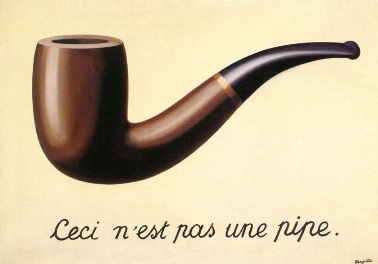
\includegraphics[width=.3\linewidth]{graphics/MagrittePipe}
  \caption{{\em The Treachery of Images} from Ren\'e Magritte}
  \label{fig:Magritte}
\end{figure}

Ren\'e Magritte painted Figure~\ref{fig:Magritte}
\end{verbatim}
}
\end{block}
\begin{figure}[ht]
  \def\figurename{Figure 1} %% a little trick 'cause beamer just
                            %% writes Figure : which makes sense in a
                            %% talk 
  \centering
  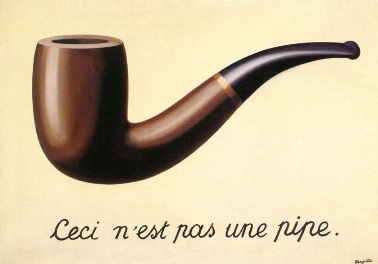
\includegraphics[width=.3\linewidth]{graphics/MagrittePipe}
  \caption{{\em The Treachery of Images} from Ren\'e
    Magritte}\label{fig:Magritte}
\end{figure}
Ren\'e Magritte painted Figure~\ref{fig:Magritte}
\end{frame}

\begin{frame}[fragile]
  \ft{Floating Objects}
  \fst{The {\tt subcaption} package}
  The {\tt subcaption} package permits to define subfloats within a
  single float
  \begin{block}{Example}
    \lstset{language=tex}
    {\scriptsize
\begin{lstlisting}
\begin{figure}
  \begin{subfigure}[b]{0.45\linewidth}
    \centering
    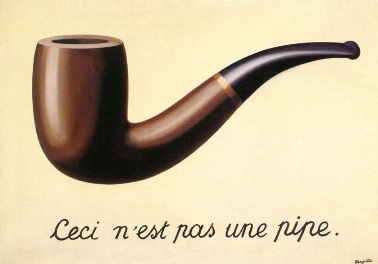
\includegraphics[width = \linewidth]{graphics/MagrittePipe}
    \caption{{\em The Treachery of Images} from Ren\'e
      Magritte}\label{sfig:magritte}
  \end{subfigure}
  \begin{subfigure}[b]{.45\linewidth}
    \centering
    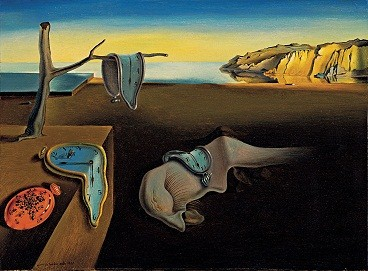
\includegraphics[width = \linewidth]{graphics/The_Persistence_of_Memory.jpg}
    \caption{{\em The Persistence of Memory} from Salvador
      Dal\'i}\label{sfig:dali}
  \end{subfigure}
  \caption{Two surrealist paintings}\label{fig:surreal}
  \end{figure}

  Do you prefer painting~\ref{sfig:magritte} or \ref{sfig:dali} from
  the two paintings presented in Figure~\ref{fig:surreal}
\end{lstlisting}
      }
  \end{block}
\end{frame}

\begin{frame}[fragile]
  \ft{Floating Objects}
  \fst{The {\tt subcaption} package}  
\begin{figure}
  \begin{subfigure}[b]{0.45\linewidth}
    \centering
    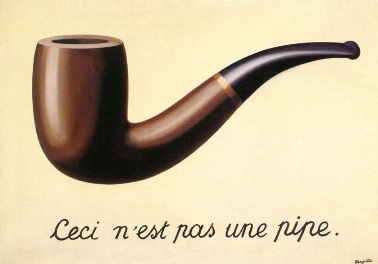
\includegraphics[width = \linewidth]{graphics/MagrittePipe}
    \caption{{\em The Treachery of Images} from Ren\'e
      Magritte}\label{sfig:magritte}
  \end{subfigure}
  \begin{subfigure}[b]{.45\linewidth}
    \centering
    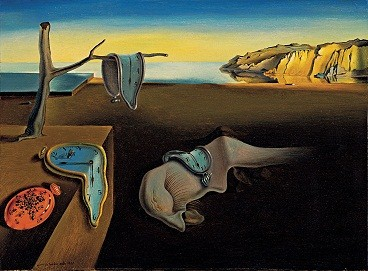
\includegraphics[width = \linewidth]{graphics/The_Persistence_of_Memory.jpg}
    \caption{{\em The Persistence of Memory} from Salvador
      Dal\'i}\label{sfig:dali}
  \end{subfigure}
  \caption{Two surrealist paintings}\label{fig:surreal}
  \end{figure}
  
  Do you prefer painting~\ref{sfig:magritte} or \ref{sfig:dali} from
  the two paintings presented in Figure~\ref{fig:surreal}
\end{frame}

\begin{frame}[fragile]
  \ft{Floating Objects}
  \fst{{\bf knitr} and {\tt subcaption}}
{\bf knitr} ($\geq 1.5$) supports the {\tt subcaption} package 
\begin{itemize}
\item Needs 
  {\scriptsize \verb|\newcommand{\subfloat}[2][need a sub-caption]{\subcaptionbox{#1}{#2}}|} \\
  in the preamble
\end{itemize}
\begin{block}{}
\begin{verbatim}
<<subfig, echo=FALSE, fig.cap = "Two histograms", 
   fig.subcap=c("Histogram for x", "histogram for y"), 
   out.width=".45\\linewidth">>=
set.seed(11111)
x <- rnorm(100)
y <- rnorm(100)

hist(x)
hist(y)
\end{verbatim}
\end{block}
\end{frame}

\begin{frame}[fragile]
  \ft{Floating Objects}
  \fst{{\bf knitr} and {\tt subcaption}}
  
\begin{knitrout}
\definecolor{shadecolor}{rgb}{0.969, 0.969, 0.969}\color{fgcolor}\begin{figure}
\subfloat[Histogram for x\label{fig:subfig1}]{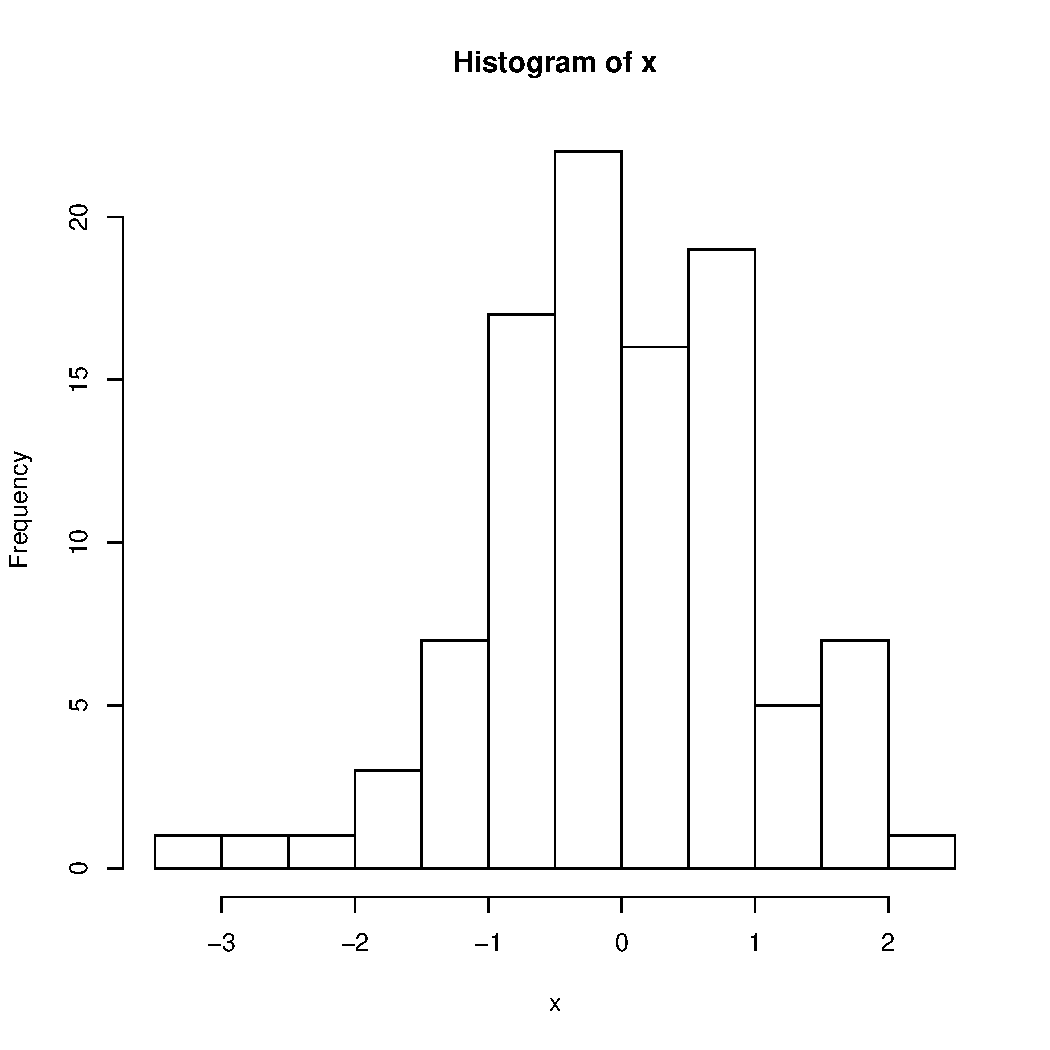
\includegraphics[width=.45\linewidth]{graphics/subfig-1} }
\subfloat[histogram for y\label{fig:subfig2}]{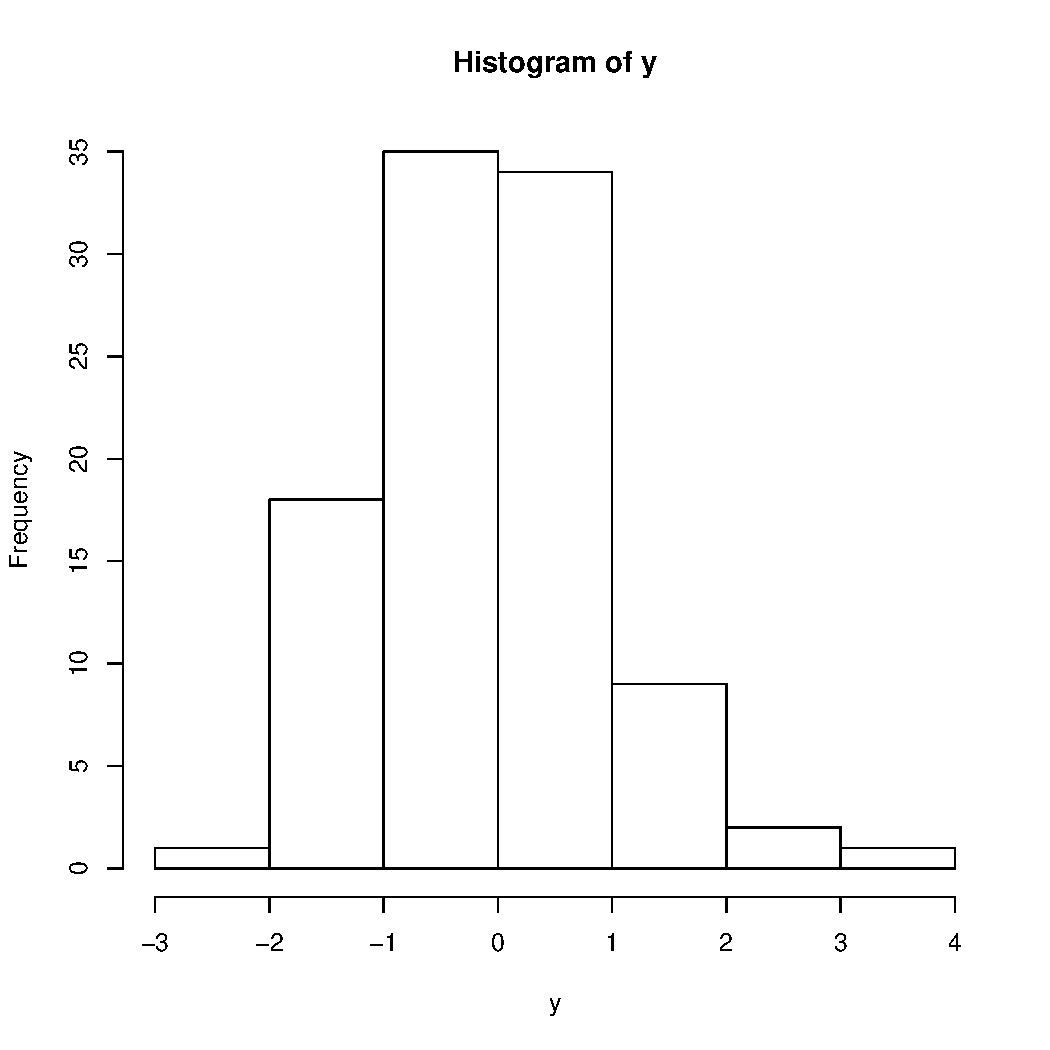
\includegraphics[width=.45\linewidth]{graphics/subfig-2} }\caption[Two histograms]{Two histograms}\label{fig:subfig}
\end{figure}


\end{knitrout}

\end{frame}

\begin{frame}[fragile]
  \ft{Floating Objects}
  \fst{The {\tt table} environment}
  \begin{columns}
    \begin{column}{5cm}
{\scriptsize
\begin{verbatim}
\begin{table}[h]
  \caption{A table}\label{tab:tab_reg}
\begin{tabular}{lccc}
\toprule
& \multicolumn{3}{c}{Regression} \\
\cmidrule(r){2-4}
& Coef & SE    & p-value         \\
\midrule
Age    & 0.01 & 0.002 & 0.5      \\
Gender & 2    & 1     & 0.23     \\
\bottomrule
\end{tabular}
\end{table}
\end{verbatim}}
    \end{column}
    \begin{column}{5cm}
\begin{table}[h]
  \caption{A table}\label{tab:tab_reg}
\begin{tabular}{lccc}
\toprule
& \multicolumn{3}{c}{Regression} \\
\cmidrule(r){2-4}
& Coef & SE    & p-value         \\
\midrule
Age    & 0.01 & 0.002 & 0.5      \\
Gender & 2    & 1     & 0.23     \\
\bottomrule
\end{tabular}
\end{table}
\end{column}
  \end{columns}
  In a lot of publications, table captions are above the respective
  tables
\end{frame}

\begin{frame}[fragile]
  \ft{Floating Objects} 
  \fst{Useful table environment} 
  
  The {\tt sidewaystable} environment is provided by the package {\tt
    rotating}

  \begin{block}{}
      {\scriptsize
\begin{verbatim}
\begin{sidewaystable}[h]
  \caption{A table}\label{tab:tab_side}
  \begin{tabular}{lccc}
    \toprule
    & \multicolumn{3}{c}{Regression} \\
    \cmidrule(r){2-4}
    & Coef & SE    & p-value         \\
    \midrule
    Age    & 0.01 & 0.002 & 0.5      \\
    Gender & 2    & 1     & 0.23     \\
    \bottomrule
\end{tabular}
 end{sidewaystable}
\end{verbatim}}
\end{block}
For tables that spread over several pages, one can use the {\tt
  longtable} environment provided by the {\tt longtable} package
\end{frame}

\begin{frame}[fragile]
  \ft{Floating Objects} 
  \fst{Tips and Tricks} 
  \begin{itemize}
  \item Think about using, e.g., \verb|[!h]| to ``force'' \LaTeX{} to
    put the figure {\em here}
  \item If that does not work, move the figure around
  \item By default, \LaTeX{} requires that there be half a page of
    text on each page of floats
    \begin{itemize}
    \item smaller graphics
    \item Override this behaviour through obscure options. See
      \url{http://www.stat.berkeley.edu/users/spector/latex2e.pdf}
      p.35 (never personally tested)
    \end{itemize}
  \end{itemize}
\end{frame}

%% \section{Pictures}

%% \begin{frame}[fragile]
%%   \ft{\LaTeX{} {\tt picture} environment}
  
%%   \begin{itemize}
%%   \item The {\tt picture} environment allows programming pictures
%%     directly in \LaTeX.
%%     \begin{block}{}
%% \begin{verbatim}
%% \begin{picture}(x, y) ... \end{picture}
%% \end{verbatim}
%%     \end{block} 
%%     or
%%     \begin{block}{}
%% \begin{verbatim}
%% \begin{picture}(x, y)(x0, y0) ... \end{picture}
%% \end{verbatim}
%%     \end{block}
%%   \item {\tt x}, {\tt y}, {\tt x0}, {\tt y0} are numbers (lengths) in
%%     the unit defined by \verb|\unitlength|. It can be changed with
%%     \verb|\setlength{\unitlength}{1mm}|
%%     \begin{itemize}
%%     \item \verb=(x, y)= affects the rectangular space for the picture
%%     \item \verb=(x0, y0)= coordinates to the bottom left corner of the
%%       reserved rectangle
%%     \end{itemize}
%%   \end{itemize}
%% \end{frame}

%% \begin{frame}[fragile]
%%   \ft{\LaTeX{} {\tt picture} environment}
%% Basic drawing command is
%% \begin{block}{}
%% \begin{verbatim}
%% \put(x, y){object}
%% \end{verbatim}
%% \end{block}

%% \setlength{\unitlength}{1cm}
%% \begin{picture}(10,10)
%%   \put(10,2){\framebox(1, 1){$1$}}
%% \end{picture}

%% \end{frame}

\end{document}
